\documentclass[a4paper, 12pt]{article}

% ---------------------------------------------------------------------------
% PACOTES
% ---------------------------------------------------------------------------
\usepackage[portuges,brazil]{babel}   % hifenizacao e nomes em portugues do Brasil
\usepackage[utf8]{inputenc}           % permite acentos diretamente no fonte
\usepackage[T1]{fontenc}              % codificacao de fonte (acentos no PDF)
\usepackage{amsmath}                  % ambientes matematicos
\usepackage{indentfirst}             % indenta o primeiro paragrafo de cada secao
\usepackage{graphicx}                 % inclusao de imagens (\includegraphics)
\usepackage{float}                    % posicionamento [H] de figuras/tabelas
\usepackage{booktabs}                 % linhas de tabela mais elegantes (\toprule etc.)
\usepackage{array}                    % colunas de tabela mais flexiveis
\usepackage{tabularx}                 % tabelas que ocupam a largura do texto e quebram linha
\usepackage{ragged2e}                 % \RaggedRight com hifenizacao em colunas estreitas
\usepackage{caption}                  % legendas customizaveis
\captionsetup{font=small,labelfont=bf,skip=6pt}  % legendas menores, rotulo em negrito
\usepackage[margin=2.5cm]{geometry}   % margens
\usepackage{xcolor}                   % cores
\usepackage{enumitem}                 % listas customizadas
\usepackage[hidelinks]{hyperref}      % links internos (sumario clicavel)

\graphicspath{{figuras/}}             % pasta padrao das figuras

% Comando auxiliar: nomes de variaveis/colunas em fonte monoespacada
\newcommand{\var}[1]{\texttt{#1}}

% Padrao de qualidade das tabelas: mais respiro entre linhas e colunas
\renewcommand{\arraystretch}{1.25}    % aumenta a altura das linhas
\setlength{\tabcolsep}{6pt}           % espacamento horizontal entre colunas

% Tipos de coluna p/ tabularx:
%   L = texto alinhado a esquerda com quebra de linha e hifenizacao
%   C = centralizado com quebra de linha
%   R = numerico alinhado a direita com quebra de linha
\newcolumntype{L}{>{\RaggedRight\arraybackslash}X}
\newcolumntype{C}{>{\Centering\arraybackslash}X}
\newcolumntype{R}{>{\RaggedLeft\arraybackslash}X}

\begin{document}

% ===========================================================================
% CAPA
% ===========================================================================
\begin{titlepage}
	\begin{center}
		\Large{\textbf{UNIVERSIDADE CATÓLICA DE BRASÍLIA}}\\
		\large{Curso de Engenharia de Software}\\
		\large{Disciplina: Estatística}\\
		\vspace{95pt}

		\textbf{\LARGE{Relatório Técnico de Análise Estatística}}\\
		\vspace{12pt}
		\textbf{\Large{Estudo de Caso: SoftTech Analytics}}\\
		\vspace{6pt}
		\large{Produtividade, qualidade, prazos, custos e satisfação\\
		em projetos de desenvolvimento de software (2024--2025)}\\
		\vspace{3.5cm}
	\end{center}

	\begin{flushleft}
		\textbf{Autor (elaboração do relatório):}\\[4pt]
		RICARDO JÚNIO SANTOS MARINHO\\[10pt]
		\textbf{Demais integrantes do grupo:}\\[4pt]
		MIGUEL MADUREIRA E SILVA, JOSÉ\\
		GABRIEL DE AQUINO REIS, VINICIUS\\
		ALVES OLIVEIRA, JÔNATAS\\[10pt]
		\textbf{Professor:} GIANCARLO ANDRADE MACHADO\\
	\end{flushleft}

	\begin{center}
		\vspace{\fill}
		Brasília -- DF\\
		Junho de 2026
	\end{center}
\end{titlepage}

% ===========================================================================
% FOLHA DE ROSTO
% ===========================================================================
\begin{titlepage}
	\begin{center}
		\Large{\textbf{UNIVERSIDADE CATÓLICA DE BRASÍLIA}}\\
		\vspace{85pt}
		\textbf{\LARGE{Relatório Técnico de Análise Estatística}}\\
		\vspace{8pt}
		\large{Estudo de Caso: SoftTech Analytics}\\
	\end{center}
	\vspace{1.5cm}

	\begin{flushright}
		\begin{minipage}{0.55\textwidth}
			Relatório técnico apresentado à disciplina de Estatística do
			curso de Engenharia de Software da Universidade Católica de
			Brasília, como requisito parcial de avaliação, sob orientação
			do Prof.\ Giancarlo Andrade Machado.
		\end{minipage}
	\end{flushright}

	\vspace{1cm}
	\begin{flushright}
		\begin{minipage}{0.55\textwidth}
			\textbf{Autor (elaboração do relatório):}\\
			Ricardo Júnio Santos Marinho\\[8pt]
			\textbf{Demais integrantes:}\\
			Miguel Madureira e Silva, José\\
			Gabriel de Aquino Reis, Vinicius\\
			Alves Oliveira, Jônatas
		\end{minipage}
	\end{flushright}

	\begin{center}
		\vspace{\fill}
		Brasília -- DF\\
		Junho de 2026
	\end{center}
\end{titlepage}

% ===========================================================================
% SUMARIO
% ===========================================================================
\newpage
\tableofcontents
\thispagestyle{empty}

\newpage
\pagenumbering{arabic}

% ===========================================================================
% IDENTIFICACAO DOS INTEGRANTES
% ===========================================================================
\section{Identificação dos integrantes e divisão de responsabilidades}

O trabalho foi desenvolvido pelo grupo abaixo, sob orientação do
Prof.\ Giancarlo Andrade Machado. A consolidação e a redação do relatório, bem
como a apresentação, foram coordenadas pelo \textbf{líder do grupo}, Ricardo
Júnio Santos Marinho. A divisão de responsabilidades adotada foi:

\begin{table}[H]
\centering
\begin{tabularx}{\textwidth}{@{} l L @{}}
\toprule
\textbf{Integrante} & \textbf{Responsabilidade} \\
\midrule
\textbf{Ricardo Júnio Santos Marinho} (líder) & Coordenação geral, elaboração do
relatório, conhecimento da base (3.1), recomendações (3.7) e encerramento \\
José Miguel Madureira e Silva & Caracterização dos projetos (3.2) e análise dos
indicadores de desempenho (3.3) \\
Vinicius Gabriel de Aquino Reis & Investigação de relações entre variáveis (3.4)
e intervalos de confiança (3.5) \\
Jônatas Alves Oliveira & Testes de hipóteses (3.6) \\
\bottomrule
\end{tabularx}
\end{table}

\noindent A apresentação oral segue a mesma divisão, com o líder abrindo e
encerrando a exposição.

% ===========================================================================
% RESUMO
% ===========================================================================
\section{Resumo}

Este relatório aplica técnicas de \textbf{estatística descritiva e inferencial}
sobre uma base de \textbf{220 projetos de software} concluídos pela empresa
fictícia \emph{SoftTech Analytics} entre 2024 e 2025. Atuando como uma equipe de
consultoria contratada pela diretoria, o grupo investiga quais fatores estão
associados ao desempenho dos projetos --- produtividade, qualidade, prazos,
custos e satisfação dos clientes --- e propõe recomendações fundamentadas em
evidências.

As análises foram conduzidas em \textbf{Python} (bibliotecas \emph{pandas},
\emph{NumPy}, \emph{SciPy} e \emph{Matplotlib}) por meio de um único script
reprodutível (\var{analise.py}), adotando nível de confiança de \textbf{95\%}
e nível de significância $\alpha = 0{,}05$. Os principais achados são:

\begin{itemize}[noitemsep]
	\item Apenas \textbf{19,5\%} dos projetos são entregues no prazo
	      (IC 95\%: 14,3\% a 24,8\%);
	\item Há \textbf{estouro sistemático de custo}: o custo real supera o
	      estimado em $\approx 27\%$ em média (teste $t$ pareado, $p \approx 3\times10^{-58}$);
	\item A \textbf{metodologia influencia o cumprimento de prazo}
	      (qui-quadrado, $p = 0{,}0001$): projetos Ágeis entregam no prazo cerca
	      de 6 vezes mais que os Tradicionais;
	\item A \textbf{satisfação do cliente} é governada pela qualidade ---
	      bugs ($r=-0{,}87$), retrabalho ($r=-0{,}81$) e horas extras
	      ($r=-0{,}81$);
	\item A \textbf{experiência média da equipe} não apresentou associação
	      relevante com a redução de defeitos (resultado contraintuitivo,
	      discutido na Seção~\ref{sec:relacoes}).
\end{itemize}

% ===========================================================================
% 1. INTRODUCAO / OBJETIVO
% ===========================================================================
\section{Objetivo}

O objetivo deste trabalho é aplicar os conceitos estudados ao longo da disciplina
na análise de uma base de dados relacionada à gestão de projetos de
desenvolvimento de software. O grupo atua como uma equipe de consultoria
contratada pela empresa fictícia para avaliar aspectos relacionados à
produtividade das equipes, à qualidade dos produtos desenvolvidos, ao
cumprimento de prazos e à satisfação dos clientes.

A análise foi realizada com ferramentas computacionais adequadas, sendo
obrigatória a \textbf{interpretação} dos resultados obtidos e sua
contextualização dentro do cenário apresentado --- e não apenas a execução
mecânica de cálculos.

% ===========================================================================
% 2. CONTEXTO
% ===========================================================================
\section{Contexto}

A empresa \emph{SoftTech Analytics} atua no desenvolvimento de sistemas sob
demanda para diferentes setores do mercado (Educação, Saúde, Finanças, Varejo,
Indústria e Governo). Ao longo dos anos de \textbf{2024 e 2025} foram registrados
diversos indicadores referentes aos projetos concluídos pela organização.

A diretoria deseja compreender \textbf{quais fatores podem estar relacionados ao
desempenho dos projetos} e quais informações podem subsidiar futuras decisões
gerenciais. Para isso, foi disponibilizada uma base de dados contendo informações
sobre equipes, metodologias de desenvolvimento, complexidade dos projetos,
prazos, retrabalho, defeitos identificados, custos e satisfação dos clientes.

O foco do trabalho, portanto, não é o cálculo em si, mas a \textbf{capacidade de
usar ferramentas estatísticas para interpretar dados e apoiar a tomada de decisão}
em um contexto realista de Engenharia de Software.

% ===========================================================================
% 3. DESENVOLVIMENTO
% ===========================================================================
\section{Desenvolvimento do trabalho}

% ---------------------------------------------------------------------------
% 3.1 CONHECIMENTO DA BASE
% ---------------------------------------------------------------------------
\subsection{Conhecimento da base de dados}
\label{sec:base}

\subsubsection{Descrição geral da base}
A base refere-se à empresa \emph{SoftTech Analytics} e reúne registros de
projetos de software concluídos entre 2024 e 2025. Cada \textbf{linha
(observação) corresponde a um projeto concluído} e cada \textbf{coluna (variável)}
a um indicador registrado sobre esse projeto --- abrangendo perfil da equipe,
metodologia, complexidade, prazos, mudanças de requisitos, defeitos, retrabalho,
custos e satisfação.

\subsubsection{Quantidade de observações disponíveis}
\begin{itemize}[noitemsep]
	\item \textbf{220 observações} (220 projetos);
	\item \textbf{22 variáveis} originais (o script cria ainda 2 variáveis
	      derivadas, \var{estouro\_custo\_mil} e \var{estouro\_pct});
	\item \textbf{0 valores faltantes} --- a base está completa, não exigindo
	      tratamento de dados ausentes.
\end{itemize}

\subsubsection{Descrição e classificação das variáveis}
A classificação de uma variável segundo sua natureza estatística determina quais
técnicas podem ser aplicadas. Variáveis \textbf{qualitativas} admitem tabelas de
frequência, gráficos de barras/setores, moda e teste qui-quadrado; variáveis
\textbf{quantitativas} admitem média, desvio padrão, histograma, boxplot,
correlação, intervalo de confiança e teste $t$. Classificar errado compromete
todas as análises seguintes.

\begin{table}[H]
\centering
\caption{Classificação das 22 variáveis segundo a natureza estatística.}
\label{tab:classificacao}
\footnotesize
\begin{tabularx}{\textwidth}{@{} >{\ttfamily\footnotesize}l L L @{}}
\toprule
\normalfont\textbf{Variável} & \textbf{Descrição} & \textbf{Classificação} \\
\midrule
id\_projeto                 & Identificador único        & Identificador (não estatística) \\
ano\_conclusao              & Ano de conclusão           & Qualitativa ordinal (temporal) \\
setor\_cliente              & Setor do cliente           & Qualitativa nominal \\
metodologia                 & Metodologia                & Qualitativa nominal \\
equipe                      & Equipe responsável         & Qualitativa nominal \\
porte\_projeto              & Porte do projeto           & Qualitativa ordinal \\
complexidade                & Complexidade técnica       & Qualitativa ordinal \\
num\_desenvolvedores        & Nº de desenvolvedores      & Quantitativa discreta \\
experiencia\_media\_anos    & Experiência média          & Quantitativa contínua \\
duracao\_planejada\_dias    & Duração prevista           & Quantitativa discreta \\
duracao\_real\_dias         & Duração real               & Quantitativa discreta \\
atraso\_dias                & Real $-$ planejada         & Quantitativa discreta (pode ser negativa) \\
mudancas\_requisitos        & Nº de mudanças             & Quantitativa discreta \\
horas\_extras               & Total de horas extras      & Quantitativa contínua \\
bugs\_total                 & Total de bugs              & Quantitativa discreta \\
bugs\_criticos              & Bugs críticos              & Quantitativa discreta \\
tempo\_medio\_correcao\_horas & Tempo médio de correção  & Quantitativa contínua \\
retrabalho\_horas           & Horas de retrabalho        & Quantitativa contínua \\
custo\_estimado\_mil        & Custo estimado (mil R\$)   & Quantitativa contínua \\
custo\_real\_mil            & Custo real (mil R\$)       & Quantitativa contínua \\
satisfacao\_cliente         & Nota de satisfação (0--10) & Quantitativa (escala) \\
entregue\_no\_prazo         & Entregue no prazo?         & Qualitativa nominal (binária) \\
\bottomrule
\end{tabularx}
\end{table}

\paragraph{Casos de fronteira.} Alguns pontos merecem discussão por
demonstrarem domínio do conceito:
\begin{itemize}[noitemsep]
	\item \var{ano\_conclusao} é numérico, mas representa um \textbf{rótulo
	      temporal}; tirar ``média de ano'' não faz sentido, por isso é tratado
	      como qualitativa ordinal.
	\item \var{satisfacao\_cliente} é uma \textbf{escala de 0 a 10}. Como aparece
	      com casas decimais e dela serão extraídas média, desvio e intervalo de
	      confiança, é \textbf{tratada como quantitativa} (registra-se, por rigor,
	      que tecnicamente é variável em escala).
	\item \var{id\_projeto}, embora numérico, é apenas um \textbf{identificador} e
	      não entra em nenhuma análise.
	\item \var{atraso\_dias} pode assumir \textbf{valores negativos} (entrega
	      antecipada), o que é estatisticamente válido e relevante.
\end{itemize}

\begin{table}[H]
\centering
\caption{Síntese da contagem de variáveis por tipo.}
\label{tab:sintese-tipos}
\begin{tabularx}{\textwidth}{@{} l c L @{}}
\toprule
\textbf{Tipo} & \textbf{Qtd.} & \textbf{Variáveis} \\
\midrule
Qualitativa nominal          & 4 & setor, metodologia, equipe, entregue\_no\_prazo \\
Qualitativa ordinal          & 3 & ano, porte, complexidade \\
Quantitativa discreta        & 7 & nº desenv., durações, atraso, mudanças, bugs \\
Quantitativa contínua        & 6 & experiência, horas extras, correção, retrabalho, custos \\
Escala (tratada como quant.) & 1 & satisfação \\
Identificador                & 1 & id\_projeto \\
\bottomrule
\end{tabularx}
\end{table}

% ---------------------------------------------------------------------------
% 3.2 CARACTERIZACAO
% ---------------------------------------------------------------------------
\subsection{Caracterização dos projetos analisados}
\label{sec:caracterizacao}

Esta seção usa estatística descritiva e gráficos para caracterizar os 220
projetos. Cada resultado vem acompanhado de discussão.

\paragraph{Porte dos projetos.}
A carteira é dominada por projetos de porte \textbf{Médio (97; 44,1\%)} e
\textbf{Pequeno (89; 40,5\%)}, que juntos somam \textbf{84,6\%}. Projetos
Grandes são minoria (34; 15,5\%). A empresa opera majoritariamente em pequena e
média escala --- os poucos grandes tendem a concentrar custos/prazos elevados e
aparecem como \emph{outliers}.

\paragraph{Metodologias.}
A metodologia \textbf{Ágil é predominante (97; 44,1\%)}, seguida da Tradicional
(75; 34,1\%) e da Híbrida (48; 21,8\%). Há adoção majoritária de práticas ágeis,
mas mais de um terço ainda segue o modelo tradicional --- divisão relevante,
pois a Seção~\ref{sec:testes} mostra que a metodologia está associada ao prazo.

\paragraph{Perfil das equipes.}
A distribuição entre as seis equipes é equilibrada (todas entre 15,0\% e 18,6\%):
Beta (41), Gamma (39), Omega (36), Sigma (36), Delta (35) e Alpha (33). Esse
balanceamento favorece comparações de desempenho sem distorção por volume.

\paragraph{Experiência média dos desenvolvedores.}
A experiência média é de \textbf{4,28 anos} (mediana 4,30; desvio 1,45), com
distribuição \textbf{aproximadamente simétrica} (assimetria $\approx 0{,}04$) e
coeficiente de variação de 34,0\%. As equipes são relativamente homogêneas,
variando de 0,8 a 9,1 anos.

\paragraph{Complexidade.}
Concentra-se em \textbf{Média (81; 36,8\%)} e \textbf{Alta (68; 30,9\%)};
\textbf{Muito alta} é rara (15; 6,8\%), mas, como se verá, está fortemente
associada a atraso, retrabalho, custo e queda de satisfação.

\paragraph{Demais características.}
Os \textbf{setores} são bem distribuídos (Governo 18,6\%; demais entre 15\% e
16,8\%); os projetos dividem-se quase igualmente entre \textbf{2025} (114; 51,8\%)
e \textbf{2024} (106; 48,2\%); o \textbf{tamanho de equipe} tem média 7,06
desenvolvedores (mediana 6) com assimetria positiva (+1,01).

\begin{figure}[H]
\centering
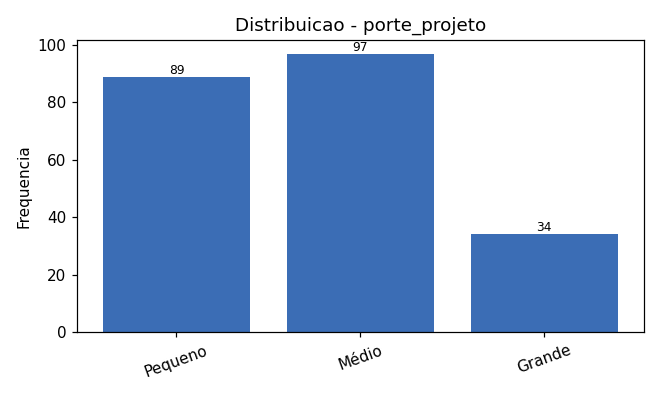
\includegraphics[width=0.48\textwidth]{barra_porte_projeto.png}\hfill
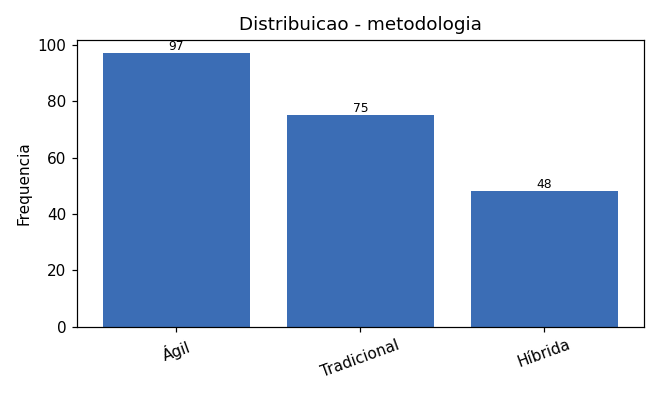
\includegraphics[width=0.48\textwidth]{barra_metodologia.png}
\caption{Distribuição do porte dos projetos e das metodologias utilizadas.}
\end{figure}

\begin{figure}[H]
\centering
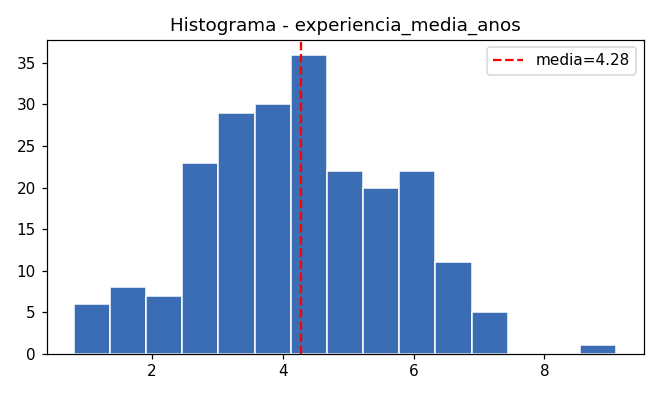
\includegraphics[width=0.48\textwidth]{hist_experiencia_media_anos.png}\hfill
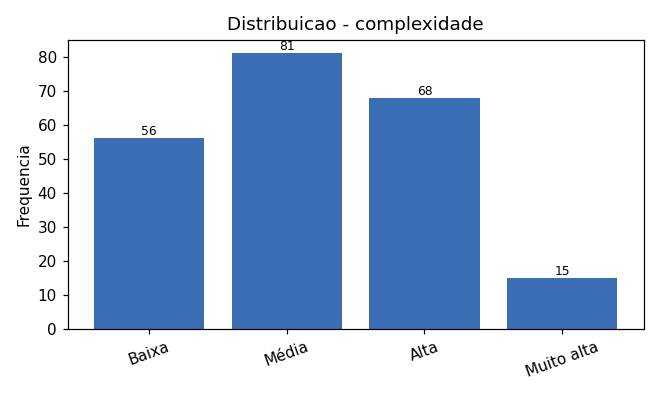
\includegraphics[width=0.48\textwidth]{barra_complexidade.png}
\caption{Experiência média das equipes (histograma) e complexidade dos projetos.}
\end{figure}

% ---------------------------------------------------------------------------
% 3.3 INDICADORES DE DESEMPENHO
% ---------------------------------------------------------------------------
\subsection{Análise dos indicadores de desempenho}
\label{sec:desempenho}

A Tabela~\ref{tab:desc} resume as principais variáveis de desempenho ($n = 220$).

\begin{table}[H]
\centering
\caption{Estatística descritiva dos indicadores de desempenho ($n=220$).}
\label{tab:desc}
\small
\setlength{\tabcolsep}{5pt}
\begin{tabular}{@{} l rrrrrrrr @{}}
\toprule
\textbf{Indicador} & \textbf{Média} & \textbf{Med.} & \textbf{D.P.} & \textbf{CV\%} & \textbf{Mín} & \textbf{Máx} & \textbf{Assim.} & \textbf{Out.} \\
\midrule
Duração planejada (dias) & 127,9 & 121,5 & 56,7 & 44,3 & 35 & 303 & $+0{,}79$ & 2 \\
Duração real (dias)      & 145,5 & 136,0 & 70,7 & 48,6 & 28 & 381 & $+0{,}81$ & 4 \\
Atraso (dias)            & 17,5 & 16,0 & 22,1 & \textbf{126,3} & $-34$ & 111 & $+0{,}98$ & 9 \\
Horas extras             & 96,6 & 88,6 & 56,8 & 58,8 & 0 & 290,9 & $+0{,}76$ & 4 \\
Retrabalho (horas)       & 162,0 & 160,0 & 83,9 & 51,8 & 0 & 421 & $+0{,}36$ & 1 \\
Bugs total               & 30,8 & 29,0 & 17,4 & 56,5 & 0 & 86 & $+0{,}39$ & 1 \\
Bugs críticos            & 4,8 & 4,0 & 4,0 & 84,2 & 0 & 17 & $+0{,}89$ & 5 \\
Custo estimado (mil R\$) & 245,0 & 220,9 & 132,2 & 54,0 & 68,9 & 672,1 & $+1{,}17$ & 13 \\
Custo real (mil R\$)     & 309,8 & 280,2 & 162,2 & 52,4 & 68,3 & 784,9 & $+0{,}99$ & 12 \\
Satisfação (0--10)       & 6,3 & 6,4 & 1,8 & 28,6 & 1,1 & 9,4 & $\mathbf{-0{,}69}$ & 8 \\
\bottomrule
\end{tabular}

\vspace{2pt}
{\footnotesize D.P.\ = desvio padrão; CV\% = coeficiente de variação;
Assim.\ = assimetria; Out.\ = nº de \emph{outliers} (regra 1,5$\times$IQR).}
\end{table}

\paragraph{Discussão.}
\begin{itemize}[noitemsep]
	\item \textbf{Prazos e atraso.} A duração real (145,5 dias) supera
	      sistematicamente a planejada (127,9). O atraso médio é de 17,5 dias, mas
	      com \textbf{dispersão altíssima (CV = 126\%)} e amplitude de $-34$ a
	      $+111$ dias. Os \textbf{9 outliers} acima de 64 dias são os casos que
	      mais merecem atenção da diretoria.
	\item \textbf{Esforço e qualidade.} Horas extras (96,6 h) e retrabalho (162 h)
	      são elevados, sinalizando sobrecarga. Cada projeto acumula em média
	      $\approx 31$ bugs, dos quais $\approx 5$ críticos.
	\item \textbf{Custos.} O custo real médio (309,8 mil) é $\approx 26\%$ maior
	      que o estimado (245,0). Ambos têm forte assimetria positiva e muitos
	      outliers superiores, puxados pelos grandes projetos.
	\item \textbf{Satisfação.} É a única variável com \textbf{assimetria negativa
	      ($-0{,}69$)}: a maioria dos clientes dá notas medianas-altas (mediana
	      6,4), mas há uma cauda de \textbf{8 projetos com notas baixas} (até 1,1)
	      que derruba a média.
\end{itemize}

\textbf{Padrão geral:} os indicadores ``ruins'' (atraso, horas extras, bugs,
custo) têm forte dispersão e cauda à direita, enquanto a satisfação tem cauda à
esquerda. Isso sugere que \textbf{um subgrupo de projetos problemáticos} concentra
os piores resultados --- hipótese reforçada pelas correlações da
Seção~\ref{sec:relacoes}.

\begin{figure}[H]
\centering
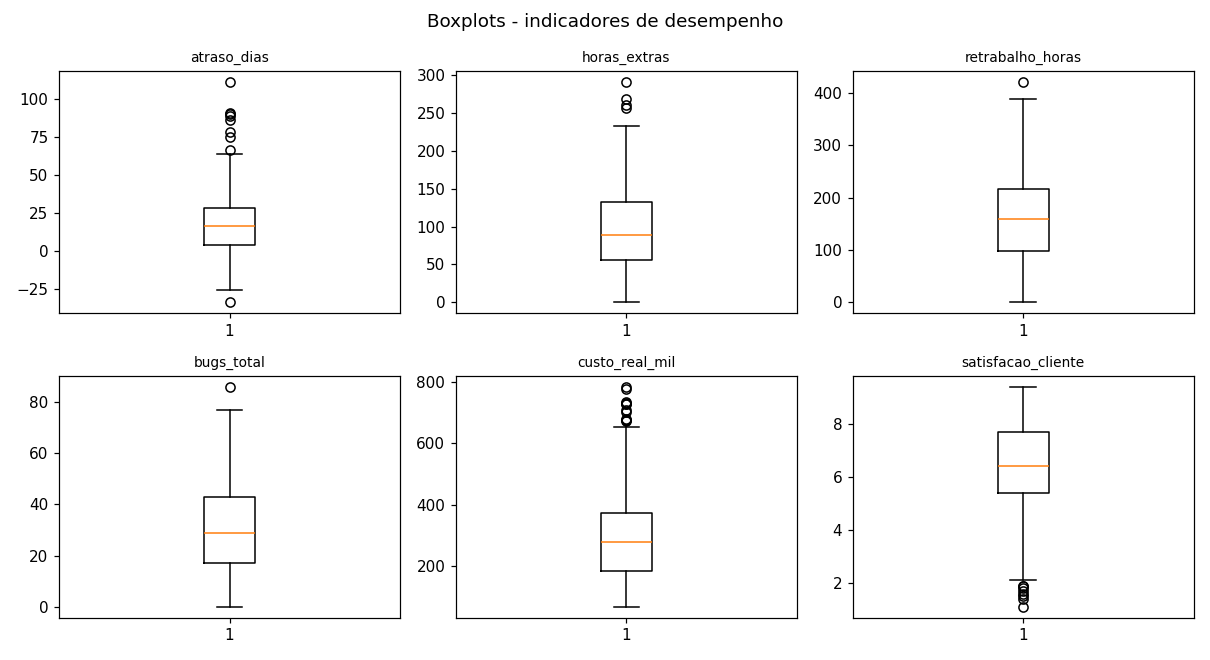
\includegraphics[width=0.85\textwidth]{boxplots_desempenho.png}
\caption{Boxplots dos indicadores de desempenho. Note a presença de
\emph{outliers} superiores em atraso, custo e horas extras, e inferiores em
satisfação.}
\end{figure}

% ---------------------------------------------------------------------------
% 3.4 RELACOES
% ---------------------------------------------------------------------------
\subsection{Investigação de relações entre variáveis}
\label{sec:relacoes}

Para cada par usou-se o coeficiente de \textbf{Pearson} (relação linear) e, como
verificação robusta, \textbf{Spearman} (relação monótona, por postos).

\begin{table}[H]
\centering
\caption{Correlações de interesse sugeridas pelo roteiro.}
\label{tab:correlacoes}
\begin{tabularx}{\textwidth}{@{} L r r L @{}}
\toprule
\textbf{Relação investigada} & \textbf{$r$ (Pearson)} & \textbf{$p$-valor} & \textbf{Conclusão} \\
\midrule
Experiência $\times$ bugs total & $-0{,}12$ & $0{,}065$     & Sem associação significativa \\
Complexidade $\times$ atraso    & $+0{,}63$ & $<0{,}0001$   & Positiva forte \\
Retrabalho $\times$ satisfação  & $-0{,}81$ & $<0{,}0001$   & Negativa forte \\
Horas extras $\times$ atraso    & $+0{,}83$ & $<0{,}0001$   & Positiva forte \\
Bugs total $\times$ satisfação  & $-0{,}87$ & $<0{,}0001$   & Negativa muito forte \\
Custo real $\times$ nº desenv.  & $+0{,}81$ & $<0{,}0001$   & Positiva forte \\
\bottomrule
\end{tabularx}
\end{table}

Relações categórica $\times$ quantitativa (via comparação de grupos):
\begin{itemize}[noitemsep]
	\item \textbf{Horas extras $\times$ prazo:} média 49,8 h (no prazo) vs
	      \textbf{107,9 h (atrasados)} --- horas extras aparecem como
	      \emph{reação} ao atraso, não como solução.
	\item \textbf{Porte $\times$ custo:} Pequeno 172,8 $\to$ Médio 330,9 $\to$
	      \textbf{Grande 608,3} mil R\$ (ANOVA $F \approx 504$): projetos grandes
	      custam em média $\approx 3{,}5\times$ mais que os pequenos.
\end{itemize}

\paragraph{Discussão.}
\begin{itemize}[noitemsep]
	\item \textbf{Experiência não reduz defeitos (contraintuitivo).} A correlação
	      é fraca e \textbf{não significativa} ($r=-0{,}12$; $p=0{,}065$). A
	      qualidade parece depender mais da \textbf{complexidade do projeto} do que
	      da senioridade da equipe.
	\item \textbf{A complexidade é o motor dos problemas.} Associa-se fortemente a
	      atraso ($r=0{,}63$); mais horas extras $\to$ mais atraso ($r=0{,}83$);
	      mais bugs/retrabalho $\to$ menos satisfação.
	\item \textbf{Qualidade é o que o cliente sente.} A satisfação é governada por
	      \textbf{bugs ($r=-0{,}87$)} e retrabalho ($r=-0{,}81$).
	\item \textbf{Custo escala com porte e tamanho de equipe} ($r=0{,}81$).
\end{itemize}

\begin{quote}
\textbf{Cautela com causalidade.} Quase todas as variáveis de desempenho são
fortemente correlacionadas entre si, provavelmente por compartilharem um
\textbf{fator latente de complexidade/porte}. As correlações indicam
\emph{associação}, não causa direta.
\end{quote}

\begin{figure}[H]
\centering
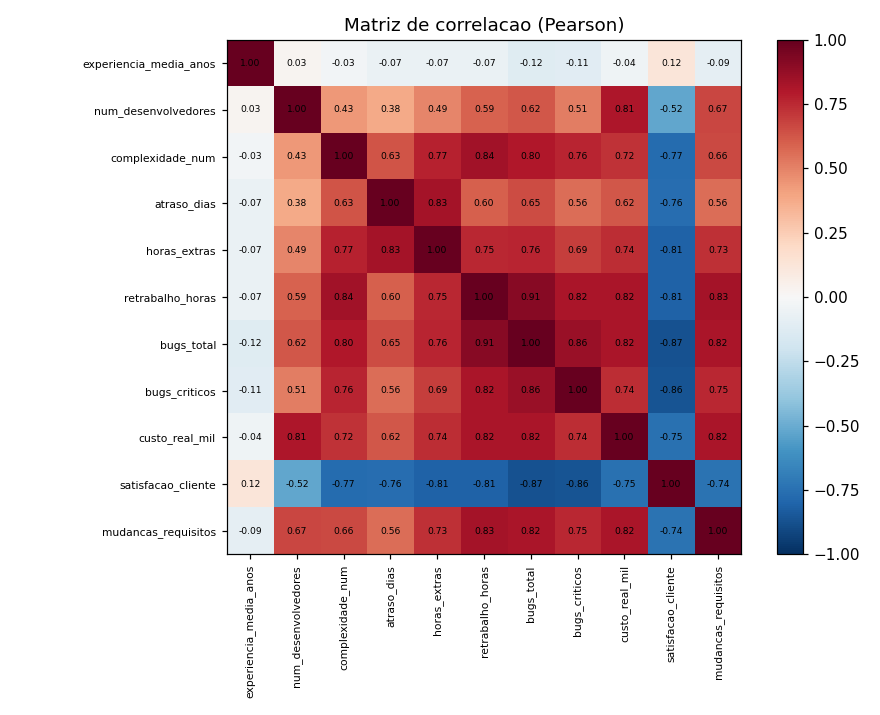
\includegraphics[width=0.7\textwidth]{heatmap_correlacao.png}
\caption{Matriz de correlação de Pearson. O bloco de variáveis de
esforço/qualidade/custo é fortemente correlacionado; a experiência da equipe
destaca-se por correlações próximas de zero.}
\end{figure}

\begin{figure}[H]
\centering
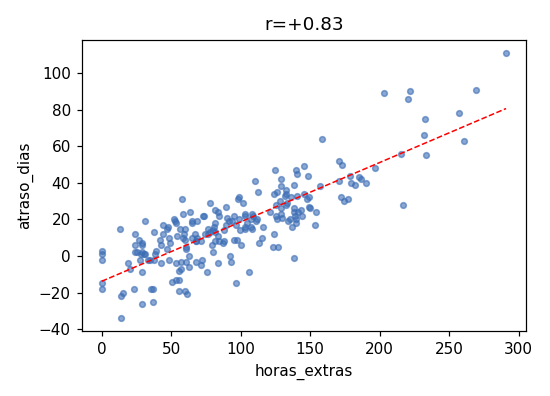
\includegraphics[width=0.48\textwidth]{scatter_horas_extras__atraso_dias.png}\hfill
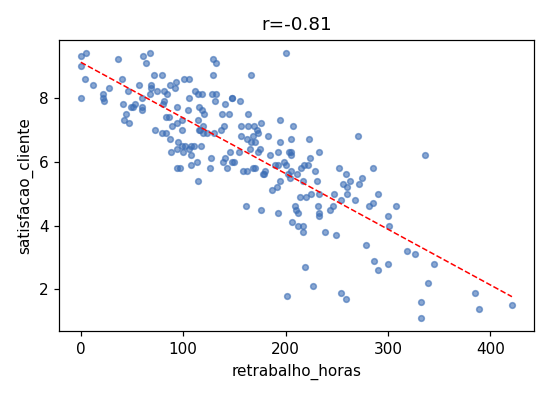
\includegraphics[width=0.48\textwidth]{scatter_retrabalho_horas__satisfacao_cliente.png}
\caption{Dispersões: horas extras $\times$ atraso ($r=+0{,}83$) e retrabalho
$\times$ satisfação ($r=-0{,}81$).}
\end{figure}

% ---------------------------------------------------------------------------
% 3.5 INTERVALOS DE CONFIANCA
% ---------------------------------------------------------------------------
\subsection{Intervalos de confiança (95\%)}
\label{sec:ic}

\paragraph{IC 1 --- Média da satisfação do cliente ($t$ de Student).}
A satisfação é o indicador-síntese da percepção do cliente. Como o desvio
populacional $\sigma$ é desconhecido, usa-se a distribuição $t$ com
$n-1 = 219$ graus de liberdade.
\[
\bar{x} = 6{,}286;\quad s = 1{,}798;\quad n = 220;\quad t_{0{,}025;\,219} = 1{,}971;
\quad \text{margem} = \pm 0{,}239
\]
\[
\boxed{\text{IC 95\%} = [\,6{,}05\,;\,6{,}53\,]}
\]
\emph{Interpretação:} com 95\% de confiança, a satisfação média da carteira está
entre \textbf{6,05 e 6,53} --- patamar apenas mediano (escala 0--10), com clara
margem de melhoria.

\paragraph{IC 2 --- Proporção de projetos entregues no prazo (aprox.\ Normal).}
Cumprimento de prazo é meta gerencial central.
\[
\hat{p} = 0{,}1955\ (43/220);\quad Z_{0{,}025} = 1{,}96;\quad \text{margem} = \pm 0{,}052
\]
\[
\boxed{\text{IC 95\%} = [\,14{,}3\%\,;\,24{,}8\%\,]}
\]
\emph{Interpretação:} com 95\% de confiança, \textbf{no máximo cerca de 1 em 4
projetos} é entregue no prazo. Mesmo no cenário mais otimista do intervalo, a
pontualidade é baixa --- um problema \textbf{estrutural}, não pontual.

\paragraph{IC 3 (apoio) --- Média do estouro de custo.}
\[
\bar{x} = 64{,}81\ \text{mil R\$};\quad \boxed{\text{IC 95\%} = [\,59{,}1\,;\,70{,}6\,]\ \text{mil R\$}}
\]
\emph{Interpretação:} em média, cada projeto custa entre \textbf{59 e 71 mil reais
a mais} que o estimado --- base quantitativa para a recomendação sobre revisão da
orçamentação.

% ---------------------------------------------------------------------------
% 3.6 TESTES DE HIPOTESES
% ---------------------------------------------------------------------------
\subsection{Testes de hipóteses ($\alpha = 0{,}05$)}
\label{sec:testes}

\subsubsection*{Teste 1 --- O custo real supera o estimado? ($t$ pareado)}
\begin{itemize}[noitemsep]
	\item \textbf{Objetivo:} verificar estouro sistemático de orçamento.
	\item \textbf{H$_0$:} $\mu_{\text{dif}} = 0$ (real $=$ estimado).
	      \quad\textbf{H$_1$:} $\mu_{\text{dif}} > 0$ (real maior).
	\item \textbf{Nível de significância:} $\alpha = 0{,}05$ (unilateral à direita).
	\item \textbf{Resultado:} diferença média $= 64{,}81$ mil R\$;
	      $t = 22{,}17$; \textbf{$p \approx 3{,}4\times10^{-58}$}.
	\item \textbf{Decisão e interpretação:} \textbf{rejeita-se H$_0$}. Há forte
	      evidência de estouro \emph{sistemático} de custo --- não é variação
	      aleatória. Em média os projetos custam $\approx 27\%$ acima do orçado,
	      indicando falha na fase de estimativa.
\end{itemize}

\subsubsection*{Teste 2 --- A metodologia influencia a entrega no prazo? (qui-quadrado)}
\begin{itemize}[noitemsep]
	\item \textbf{Objetivo:} testar associação entre metodologia e prazo.
	\item \textbf{H$_0$:} metodologia e prazo são independentes.
	      \quad\textbf{H$_1$:} são associadas.
	\item \textbf{Nível de significância:} $\alpha = 0{,}05$.
\end{itemize}

\begin{table}[H]
\centering
\caption{Tabela de contingência observada: metodologia $\times$ entrega no prazo.}
\label{tab:contingencia}
\begin{tabular}{@{} l c c c @{}}
\toprule
\textbf{Metodologia} & \textbf{Não} & \textbf{Sim} & \textbf{\% no prazo} \\
\midrule
Ágil        & 67 & 30 & \textbf{30,9\%} \\
Híbrida     & 39 & 9  & 18,8\% \\
Tradicional & 71 & 4  & \textbf{5,3\%} \\
\bottomrule
\end{tabular}
\end{table}

\begin{itemize}[noitemsep]
	\item \textbf{Resultado:} $\chi^2 = 17{,}65$; gl $= 2$; \textbf{$p = 0{,}0001$}.
	\item \textbf{Decisão e interpretação:} \textbf{rejeita-se H$_0$}. A
	      metodologia está \emph{associada} ao cumprimento de prazo: projetos Ágeis
	      entregam no prazo $\approx 6\times$ mais que os Tradicionais
	      (30,9\% vs 5,3\%) --- evidência forte a favor de práticas ágeis.
\end{itemize}

\subsubsection*{Teste 3 (extra) --- A satisfação difere entre metodologias? (ANOVA)}
\begin{itemize}[noitemsep]
	\item \textbf{Objetivo:} verificar se a satisfação média varia com a metodologia.
	\item \textbf{H$_0$:} $\mu_{\text{Ágil}} = \mu_{\text{Híbrida}} = \mu_{\text{Tradicional}}$.
	      \quad\textbf{H$_1$:} ao menos uma difere.
	\item \textbf{Resultado:} médias --- Ágil 6,73; Híbrida 6,28; Tradicional 5,72;
	      $F = 6{,}98$; \textbf{$p = 0{,}0012$}.
	\item \textbf{Decisão e interpretação:} \textbf{rejeita-se H$_0$}. A satisfação
	      difere entre metodologias, sendo mais alta na Ágil e mais baixa na
	      Tradicional --- coerente com o resultado de prazo do Teste 2.
\end{itemize}

% ---------------------------------------------------------------------------
% 3.7 RECOMENDACOES
% ---------------------------------------------------------------------------
\subsection{Recomendações para a diretoria}
\label{sec:recomendacoes}

Com base nas evidências estatísticas apresentadas:

\begin{enumerate}[leftmargin=*]
	\item \textbf{Rever o processo de estimativa de custos.} O estouro é
	      sistemático e significativo (Teste 1; IC de $+59$ a $+71$ mil R\$ por
	      projeto). Incorporar margens de contingência calibradas por porte e
	      complexidade e revisar as premissas de orçamentação.
	\item \textbf{Expandir o uso de metodologias ágeis.} Projetos Ágeis entregam
	      no prazo $\approx 6\times$ mais que os Tradicionais (Teste 2) e têm maior
	      satisfação (Teste 3). Migrar projetos Tradicionais para abordagens
	      ágeis/híbridas tende a melhorar prazo e satisfação simultaneamente.
	\item \textbf{Atacar a pontualidade como problema estrutural.} Apenas 14--25\%
	      dos projetos saem no prazo (Seção~\ref{sec:ic}). Rever o planejamento de
	      prazos e a gestão de horas extras --- que estão associadas a \emph{mais}
	      atraso (107,9 h nos atrasados vs 49,8 h nos pontuais).
	\item \textbf{Priorizar a redução de defeitos para elevar a satisfação.} Bugs
	      e retrabalho são os maiores determinantes da insatisfação ($r=-0{,}87$ e
	      $-0{,}81$). Investir em testes, revisão de código e qualidade tende a ter
	      o maior retorno em satisfação.
	\item \textbf{Gerenciar a complexidade com atenção redobrada.} É o fator de
	      fundo que eleva atraso, retrabalho e custo. Projetos de complexidade
	      ``Muito alta'' (apenas 6,8\% da base) devem receber alocação reforçada e
	      acompanhamento próximo desde o início.
\end{enumerate}

\begin{quote}
\textbf{Ressalva metodológica:} as relações encontradas são associações
estatísticas, não necessariamente causais. As recomendações apontam direções
fundamentadas nos dados, que devem ser validadas com conhecimento de negócio
antes de mudanças de larga escala.
\end{quote}

% ===========================================================================
% 4. SOBRE A FERRAMENTA / CODIGO
% ===========================================================================
\section{Sobre a ferramenta computacional e o código}
\label{sec:codigo}

Toda a análise foi automatizada em um único script Python (\var{analise.py}),
garantindo \textbf{reprodutibilidade}: executando \var{python analise.py} a
partir da raiz do projeto, o programa lê o arquivo Excel original e
(re)gera as pastas \var{figuras/} (gráficos PNG) e \var{saidas/} (tabelas CSV e o
resumo \var{RESUMO\_analise.txt}). Rodar novamente sobrescreve as saídas com os
mesmos resultados.

\paragraph{Bibliotecas e por que foram escolhidas.}
\begin{itemize}[noitemsep]
	\item \emph{pandas} --- leitura do Excel e manipulação da tabela
	      (\texttt{DataFrame}); centraliza filtros, agrupamentos e estatísticas
	      descritivas (\texttt{describe()}, \texttt{value\_counts()}).
	\item \emph{NumPy} --- cálculos numéricos vetorizados (ex.: ajuste da reta de
	      regressão com \texttt{polyfit}, raízes quadradas dos erros-padrão).
	\item \emph{SciPy (scipy.stats)} --- núcleo inferencial: valor crítico $Z$ e
	      $t$, correlações de Pearson/Spearman, teste $t$ pareado, qui-quadrado e
	      ANOVA.
	\item \emph{Matplotlib} --- geração dos gráficos. Usa-se o backend
	      \texttt{Agg} (``sem janela'') para apenas salvar arquivos, adequado a
	      execução automatizada.
\end{itemize}

\paragraph{Principais decisões e funções do código.}
\begin{itemize}[leftmargin=*]
	\item \textbf{Parâmetros globais.} Define-se $\alpha = 0{,}05$ e nível de
	      confiança de 95\%; o valor crítico $Z \approx 1{,}96$ é obtido de
	      \texttt{st.norm.ppf}. Centralizar esses parâmetros evita inconsistências.
	\item \textbf{Correção de acentuação (\texttt{conserta}).} A planilha veio
	      codificada em \texttt{cp1252}; a função recodifica as strings para
	      \texttt{utf-8}, recuperando os acentos (ex.: ``Saúde'', ``Indústria'').
	\item \textbf{Separação por tipo (\texttt{CAT} e \texttt{NUM}).} As colunas são
	      classificadas em qualitativas e quantitativas --- exatamente a distinção
	      estatística da Seção~\ref{sec:base} ---, o que define qual técnica é
	      aplicada a cada uma.
	\item \textbf{Variáveis derivadas.} Criam-se \var{estouro\_custo\_mil}
	      (real $-$ estimado) e \var{estouro\_pct} (\% sobre o estimado), usadas no
	      IC de apoio e no Teste 1.
	\item \textbf{Descritiva.} Para as quantitativas calcula-se média, mediana,
	      desvio, coeficiente de variação (\texttt{CV\%}), assimetria e curtose.
	\item \textbf{Detecção de \emph{outliers} (regra 1,5$\times$IQR de Tukey).}
	      Valores fora de $[Q_1 - 1{,}5\,\text{IQR};\ Q_3 + 1{,}5\,\text{IQR}]$ são
	      contados por variável --- base da coluna ``Out.'' da Tabela~\ref{tab:desc}.
	\item \textbf{Funções gráficas.} \texttt{barra()} gera gráficos de barras
	      (com ordem lógica para variáveis ordinais como porte e complexidade);
	      histogramas marcam a média com linha tracejada; boxplots resumem a
	      dispersão e os outliers dos indicadores de desempenho.
	\item \textbf{Correlações.} Calcula-se a matriz de Pearson (heatmap) e, para os
	      pares de interesse, também Spearman --- a coincidência entre os dois
	      coeficientes reforça a robustez das conclusões.
	\item \textbf{Inferência.} Os ICs usam $t$ de Student (média) e aproximação
	      Normal (proporção); os testes usam \texttt{ttest\_rel} (pareado),
	      \texttt{chi2\_contingency} (qui-quadrado) e \texttt{f\_oneway} (ANOVA).
	\item \textbf{Registro (\texttt{log}).} Uma função utilitária imprime na tela e
	      acumula as linhas, salvas ao final em \var{RESUMO\_analise.txt} ---
	      garantindo rastreabilidade de todos os números citados neste relatório.
\end{itemize}

\paragraph{Foco principal da análise.}
O foco não foi a execução mecânica de cálculos, mas \textbf{identificar os fatores
que governam o desempenho dos projetos}. A investigação convergiu para três
problemas centrais e acionáveis: \textbf{(i)} o estouro sistemático de custo,
\textbf{(ii)} a baixíssima taxa de pontualidade e \textbf{(iii)} o papel da
qualidade (bugs e retrabalho) como principal determinante da satisfação ---
com a \textbf{complexidade} surgindo como fator latente por trás de quase todos
os indicadores.

% ===========================================================================
% 5. CONCLUSOES
% ===========================================================================
\section{Conclusões}

A base da \emph{SoftTech Analytics} (220 projetos, completa e equilibrada
temporalmente) revelou um portfólio predominantemente de pequeno/médio porte,
metodologia majoritariamente Ágil e equipes homogêneas em experiência. As
análises descritiva e inferencial mostraram, de forma estatisticamente
fundamentada, que:

\begin{itemize}[noitemsep]
	\item o \textbf{estouro de custo é sistemático} ($p \approx 3\times10^{-58}$),
	      com magnitude estimada entre $+59$ e $+71$ mil R\$ por projeto;
	\item a \textbf{pontualidade é estruturalmente baixa} (IC 95\%: 14,3\%--24,8\%);
	\item a \textbf{metodologia importa} para prazo e satisfação (qui-quadrado e
	      ANOVA significativos), favorecendo abordagens ágeis;
	\item a \textbf{qualidade (bugs e retrabalho) dirige a satisfação}, enquanto a
	      \textbf{experiência da equipe não reduziu defeitos} --- achado
	      contraintuitivo que redireciona a atenção para a gestão da complexidade.
\end{itemize}

As recomendações da Seção~\ref{sec:recomendacoes} traduzem esses achados em ações
gerenciais, sempre com a ressalva de que correlação não implica causalidade.

% ===========================================================================
% TRABALHOS FUTUROS
% ===========================================================================
\section{Trabalhos futuros}

Como continuidade, sugerem-se: \textbf{(i)} modelos de regressão múltipla para
isolar o efeito da complexidade dos demais indicadores; \textbf{(ii)} análise
temporal comparando 2024 e 2025 para detectar tendências; e \textbf{(iii)} testes
post-hoc (ex.: Tukey) após a ANOVA, para identificar exatamente quais metodologias
diferem entre si em satisfação.

% ===========================================================================
% REFERENCIAS
% ===========================================================================
\addcontentsline{toc}{section}{Referências}
\section*{Referências}
\footnotesize{
\noindent BUSSAB, W. O.; MORETTIN, P. A. \emph{Estatística Básica}. 9.\ ed. São Paulo: Saraiva, 2017.\\[4pt]
\noindent TRIOLA, M. F. \emph{Introdução à Estatística}. 12.\ ed. Rio de Janeiro: LTC, 2017.\\[4pt]
\noindent McKINNEY, W. \emph{Python for Data Analysis}. 3.\ ed. O'Reilly, 2022.\\[4pt]
\noindent VIRTANEN, P. et al. SciPy 1.0: Fundamental Algorithms for Scientific Computing in Python. \emph{Nature Methods}, v.\ 17, 2020.\\
}

% ===========================================================================
% ANEXOS
% ===========================================================================
\newpage
\addcontentsline{toc}{section}{Anexos}
\section*{Anexos}

\textbf{Anexo A --- Código-fonte.} O script completo de análise
(\var{analise.py}), devidamente comentado, acompanha a entrega.

\textbf{Anexo B --- Tabelas geradas (pasta \var{saidas/}).} Frequências das
qualitativas (\var{2\_freq\_*.csv}), descritiva das quantitativas
(\var{3\_descritiva\_quantitativas.csv}), outliers (\var{3\_outliers\_iqr.csv}),
matriz de correlação (\var{4\_matriz\_correlacao\_pearson.csv}), correlações de
interesse (\var{4\_correlacoes\_interesse.csv}), contingência metodologia
$\times$ prazo (\var{6\_tab\_metodologia\_prazo.csv}) e o resumo consolidado
(\var{RESUMO\_analise.txt}).

\textbf{Anexo C --- Gráficos gerados (pasta \var{figuras/}).} Barras das
qualitativas, histogramas, boxplots de desempenho, heatmap de correlação e
gráficos de dispersão dos pares de interesse.

\textbf{Anexo D --- Base de dados.} \var{Dados\_Brutos\_estatistica\_estudo\_caso
(1).xlsx} (abas \emph{Dados\_Brutos}, \emph{Dicionario} e \emph{Categorias}).

\end{document}
